
\subsection{Linear Regression \mia{copy}}\label{Linreg}
Linear regression bases itself on the assumption of a linear relationship between the \textit{predictors} and the \textit{response} \cite[p.21-26]{fahrmeir}. 
Given a data set of $p$ input variables (commonly called predictors), $X=[x_1, \, x_2, \, \ldots, \, x_p]$ and a data set of output variables (commonly called the response) one seeks a linear model on the form
\begin{equation}
\Tilde{y}=\hat{\beta_0}+\sum_{j=1}^{p}x_j\hat{\beta_j}.
\end{equation}
The scalar $\Tilde{y}$ is the prediction of the response, $\hat{\beta_0}$ the estimated intercept, and each $\hat{\beta_j}$ the estimated coefficient belonging to its corresponding predictor $x_j$. 

This equation is commonly written in vector form, 
\begin{equation}
\Tilde{\y}=\boldsymbol{X}^T\boldsymbol{\hat{\beta}},
\end{equation}

where given $n$ different sets of input/output-variables (data points), $\Tilde{\y}$ is the response-vector and $\boldsymbol{X}$ is a $n\times (p+1)$-matrix called the \textit{design matrix}\label{design-matrix}. Here the $'+1'$ column in $\boldsymbol{X}$ is a row of ones for inclusion of the intercept in $\boldsymbol{\hat{\beta}}$, and the residual $p$ columns each of the $p$ predictor variables. 


The "true" model is assumed the form 
\begin{equation}\label{OG_y}
y=\beta_0+\sum_{j=1}^{p}x_j\beta_j+\epsilon.
\end{equation}
Our linear regression models are always estimations of the equation above, and for real-life data there's no way of knowing the true $\boldsymbol{\beta}$ (for generated data there will be exceptions). 
$\epsilon$ is an irreducible \textit{error-term} or \textit{residual-term} representing all variance in the data not explainable by the linear model; any variation due to randomness is included in this term. It is assumed $\epsilon \sim  
\mathcal{N}(0,\sigma^2)$.

The main objective when solving linear regression problems, is finding the optimal coefficients $\boldsymbol{\beta}$ that minimizes an error measure between $y_i$ and $\Tilde{y_i}$. 
How such an optimal solution evinces is dictated by the definition of the \textit{cost-function},  or \textit{loss-function}, which is simply metrics chosen to measure how much the predictions deviate from the "truth". 
A cost-function, $\text{Cost}(f,\mathcal{D} )$, is used to describe such a metric measuring a group of data-points, while a loss-function, $L(y, \hat{y})$, describes a metric regarding a single data-instance. 
The cost-function can be expressed in terms of the loss function
\begin{equation}
\text{Cost}(f,\mathcal{D}) = \frac{1}{n}\sum_{i=1}^n L(y_i, \hat{y_i}),
\end{equation}
as the average of the loss-function over the data. 
Through different choices of cost-function one ends up with different methods for estimation, resulting in different models for the same data-set. 


\subsubsection{OLS\mia{copy}}

\textit{Ordinary least squares} is a linear regression method that seeks to minimize the following cost function:

\begin{equation}\label{cost_ols}
    C(\bet) = \sum_{i=0}^{n-1}(y_i-\Tilde{y}_i)^2
\end{equation}

From Eq. \ref{cost_ols} the equation for the optimal $\bet$ can be derived. This is done by taking the derivate of the cost function w.r.t. $\bet$ and finding the minimum. The optimal $\bet$ for OLS is given: 

\begin{equation}\label{betaols}
    \hat{\bet}_{\text{OLS}} = \betta = \boldsymbol{H}\y
\end{equation}

The $\boldsymbol{H}$ is popularly called the Hessian matrix. The Hessian matrix for OLS specifically is stated in Eq. \ref{betaols}, but the term ``Hessian matrix'' generally describes a square matrix of double derivatives.


Ordinary least squares provides an unbiased estimation - meaning the expected value of the estimated betas is equal to the true betas, as shown in Eq. \ref{ols}.  

\begin{equation}\label{ols}
    \fv{\hat{\bet}_{OLS}} = \bet
\end{equation}

\begin{equation}
   \text{var}(\hat{\bet}_{OLS}) = \sigma^2 (\mathbf{X}^T\mathbf{X})^{-1}
\end{equation}

OLS regression is invariant to scaling of the data.

\subsubsection{Ridge\mia{copy}}


An extension of the ordinary least squares method is to add a penalization term to the cost-function. There are many reasons why this is often preferred. 

Firstly, when OLS is performed it is assumed that the matrix $\boldsymbol{X}^T\boldsymbol{X}$ in Eq. \ref{betaols} is invertible. This may not always be the case due to correlation between the predictors in the data set, or if $p > n$. In these cases the matrix will not be full rank, i.e. not invertible. 
A mathematical fix to this is to add a (small) number $\lambda$ along the diagonal: 
\begin{equation}\label{pen}
    \hat{\bet} = (\mathbf{X}^T\mathbf{X}- \lambda\boldsymbol{I})^{-1}\mathbf{X}^T\mathbf{y}
\end{equation}

These methods also help to reduce overfitting. Intuitively this is a result of penalizing "too good of a fit" on the training data, meaning it's harder for models to get overfit. 

Eq. \ref{pen} is the general equation for the coefficients in penalized regression, where the parameter $\lambda$ controls the regularization. Among the many types of choices for penalization metrics are the L1-norm penalty, also known as Lasso, and the L2-norm penalty, known as Ridge. Different types of penalties yields in different properties and interpretations related to the resulting models.

In Ridge regression, the L2-norm penalty gives us the following cost-function:

\begin{equation}\label{ridge}
     C(\bet) = \sum_{i=0}^{n-1} \left( y_i - \sum_{j=1}^{p-1} X_{ij}\beta_j \right)^2 + \lambda\sum_{j=1}^{p-1} \beta_j^2 
\end{equation}




This can alternatively be expressed as two equations, where the restraint on $\bet$ is explicitly stated:
\begin{equation}\label{ridge_alt}
    C(\bet) = \sum_{i=1}^N \left(y_i - \sum_{j=1}^{p-1} X_{ij}\beta_j \right)^2
\end{equation}
\begin{equation}\label{ridge_constraint}
    \sum_{j=1}^p \beta_j^2 \leq t, 
\end{equation}
Here the value of t is directly related to the value of $\lambda$ \citep[p. 63]{hastie}.

Ridge regression puts a penalty on all the $\beta$-terms except the intercept, which is held out during training. Had it been included, the model would depend on the chosen origin and this dependency undermines the principle of shift invariance \citep[p. 63]{hastie}.
The value of $\beta_0$ is later calculated as Eq. \ref{bet0} \julie{denne refen må fikses eller fjernes} shows. 

In the ideal case, when the design matrix $\mathbf{X}$ is orthogonal, one has $\mathbf{X}^T\mathbf{X} = \boldsymbol{I}$. From Eq. \ref{pen} gets that:
\begin{equation}\label{ridgeOLSder}
    \bet_{Ridge} = (\boldsymbol{I} - \lambda\boldsymbol{I}) \mathbf{X}^T \mathbf{y}
\end{equation}
From Eq. \ref{ridgeOLSder}, it immediately follows that, in the case of $\mathbf{X}$ orthogonal, one gets the relation:
\begin{equation}\label{ridgeOLS}
    \bet_{Ridge} = \frac{1}{1+\lambda}\bet_{OLS}
\end{equation}

The solutions produced by Ridge regression depend on the scaling of the data. It is therefore especially important to standardize the data as explained in section \ref{sec:scaling}. \julie{denne refen må fikses eller fjernes}



\subsection{Classification \julie{??}}
\julie{this section needs major rework, might consider mentioning discriminatory vs. generativ classifiers instead idk}
% \mia{Classification versus regression must in somewhere}
% - Boils down to continuous vs. discrete
Regression is one of the two main applications in which statistical learning is used for prediction; \textit{classification} is the other. Classification aims to, evidently, model a way to classify a data-point. As one might infer the two have a lot of conceptual overlap, and in a sense they represent two sides of estimation; the continuous and the discrete \cite[p. 10]{hastie}. 
% Among typical applications we find stockmarket predictions, medical risk-classifications, and image-identification. 
Many methods for classification even utilize some of the same methods used for regression, only now including extra step(s) to classify the computations.

Similarly as with linear regression, one has a design-matrix $X$, and wishes to predict an outcome for each data-point based on these values \cite[Logistic Regression]{morten}. Only now, the goal is not a numerical value, but rather to classify data-points into one of $K$ classes. $X$ is again a $n\times p$-matrix, consisting of $n$ samples from $p$ parameters.

Some methods "force-classify", selecting and outputting a given class. One example of this is the sign-function, popularly called the Perceptron. This is a binary function, outputting 1 if the computed value is non-negative, and 0 otherwise. Here one is guaranteed a class-assignment as output. 
While this is good for some applications, one is sometimes more interested in knowing how likely it is that something belongs to a certain class - this is called \textit{soft-classifying}. Among the more common types of soft-classifiers there is \textit{logistic regression}. 

Most common classificiation task is binary. 

\subsection{Logistic Regression}
 \julie{is this okay? or still imprecise?}
Logistic regression seeks to use linear functions to model the posterior probabilities of an instance belonging to a class - while still maintaining a legal probability distribution with values ranging $[0,1]$ and summing to one \cite[p.119]{hastie}. 

In standard implementation of logistic regression one commonly works with a binary case; yes/no, true/false, $1/0$, diseased/not-diseased, etc. Through logistic regression the aim is to decide whether an instance belongs to a class, or not \cite[p. 78]{jm3}.  
Borrowing from standard linear regression, the posterior probability for class 1 given x can be expressed as:  
\begin{equation}
\Pr(G=1|X=x)=\beta_0+\beta^Tx
\end{equation} 
However, this equation yields values ranging anywhere on the real number line, and thus fulfills neither of the aforementioned criterion for the distribution. This prompts the introduction of the \textit{sigmoid function}, also called the logistic function;
\begin{equation}\label{sigmoid}
    \sigma(z)=\frac{1}{1+\exp(-z)}=\frac{\exp(z)}{1+\exp(z)}
\end{equation}

By taking values in the real numbers, and forcing them between $[0,1]$, one can ensure the former part of the distribution criteria - leaving us with the following expression for the first posterior probability. 
\begin{equation}\label{priprob1}
\Pr(G=1|X=x)=\frac{\exp(\beta_0+\beta_1x_1)}{1+\exp(\beta_0+\beta_1x_1)}
\end{equation}

The latter part of the criterion is ensured trough the definition of the second class probability;
\begin{align}\label{priprob0}
    \Pr(G=0|X=x)=&1-\Pr(G=1|X=x) \\ =& 
    \frac{1}{\exp(\beta_0+\beta_1x_1)}
\end{align}
The final step in the classifier is in many ways the simplest one; the decision with the highest probability is chosen. This will arbitrarily be the equivalent of looking only at the posterior probability of the instance belonging to the class, $P=Pr(G=1)|X=x)$ with a decision boundary of $0.5$. For $P\geq0.5$ the decision then falls to "yes", and the opposite when $P<0.5$. 
Which side of the decision the midpoint is assigned to is of no consequence to the models performance, but it is commonly set as belonging to "yes" category.



Logistic regression can be generalized for the non-binary case, which is then called \textit{multinomial logistic regression}. This generalization is done by comparing the posterior probabilities of the instance belonging to each of $K$ classes respectively. Multinomial logistic regression will not be further covered in this report. 

% The fact that the denominator contains the posterior for exactly class $K$ is arbitrary, and the relative relationship between the class-probabilities remains the same no matter what class is chosen for the denominator. 

% The posterior probability for each class can be easily derived from Eq. \ref{logpri}, and is given by Eq. \ref{postprob_k1} for $k= 1,\dots,K-1$ and Eq. \ref{postprob_k} for class $K$.  
% \begin{equation}\label{postprob_k1}
% \Pr(G=k|X=x)=\frac{\exp(\beta_{k_0}+\beta_k^Tx)}{1 + \sum_{l=1}^{K-1}\exp(\beta_{l_0}+\beta_l^Tx))}
% \end{equation}
% \begin{equation}\label{postprob_k}
% \Pr(G=K|X=x)=\frac{1}{1 + \sum_{l=1}^{K-1}\exp(\beta_{l_0}+\beta_l^Tx))}  
% \end{equation}

\subsection{Cost functions for binary classification \julie{elns}}
\julie{must remember to include maximum likelihood in theory!!}

When choosing a cost-function for the training of a classification model least squares or similar methods are no longer an option. These functions account for neither the discreteness or the non-linearity of the classification task. 
As methods like logistic regression necessitate a probabilistic interpretation of the output, one needs a cost function that reflects the probability of each class accurately. In particular, our goal is to make the predicted probabilities of the correct classes as close to 1 as possible, while minimizing the probabilities of incorrect classes. Here \textit{cross-entropy loss} becomes useful.

Entropy stems from the field of information theory, introduced as something akin to a measure of uncertainty \cite{Shore}. Building on this, cross-entropy was later proposed as a quantitative measure of how far a predicted probability distribution deviates from the true distribution that it aims to model. Provided as Eq. \ref{cross-entropy loss},
\julie{is this too "historic" for a theory section?}

\begin{equation}\label{cross-entropy loss}
    L(y, \hat{y}) = - \left( y \cdot \log(\hat{y}) + (1 - y) \cdot \log(1 - \hat{y}) \right)
\end{equation}

\begin{equation}\label{cross-entropy cost}
    C(Y, \hat{Y}) = - \frac{1}{N} \sum_{i=1}^{N} \left( y_i \cdot \log(\hat{y}_i) + (1 - y_i) \cdot \log(1 - \hat{y}_i) \right)
\end{equation}
\subsection{Gradient descent}
%morten lecture notes
\julie{need transition here, maybe natural about optimization of mentioned cost-func in last section}
In the case of linear regression and least squares (Sec. \ref{Linreg}), the optimal coefficients for minimizing the cost-function can easily be found analytically. This is however not always the case; for more complicated methods, like logistic regression and neural networks, the steps for optimizing the model are not as simple and in many cases can only be approximated numerically.  
One method for this type of numeric optimization, and arguably the most popular one, is \textit{gradient descent} (GD). In addition to benefits of efficiency and performance, gradient descents triumphs in it's versatility as it can be used for a wide range of optimization problems - including linear regression, logistic regression, neural networks, and many more. 


Imagining the graph of a cost-function as a hilly landscape; global and local minima as valleys, poorer solutions as hills - GD seeks to land in the deepest valley, i.e. the global minimum. 
By looking at the slope of the landscape one can keep taking steps in the steepest descending direction, and this way hopefully end up at this minimum.

\begin{equation}\label{eq:gd}
    -\nabla_\theta C(\theta) = -\begin{bmatrix}
\frac{\partial C}{\partial \theta_1} \\
\frac{\partial C}{\partial \theta_2} \\
\vdots \\
\frac{\partial C}{\partial \theta_n}
\end{bmatrix}
\end{equation}

More precisely, one finds the gradient of the cost-function with respect to the parameters of the model - which provides the direction of steepest increase. The negative of the gradient will then provide the direction of steepest decrease, as given for a general cost-function in Eq. \ref{eq:gd}. $\theta$ represent the entire model, while the $\theta_i$s represent each of the parameters present in the model.

\begin{equation}\label{eq:updt_std}
    \theta_{t+1} = \theta_t - \eta_t \nabla_{\theta} C(\theta_t)
\end{equation}

When updating the parameters in the model, we now use this gradient combined with a new parameter $\eta$, as shown in Eq. \ref{eq:updt_std}.
$\eta$ is commonly known as the \textit{learning rate}, which we will discuss further below.

For a model containing only a few data-points and parameters computing the gradient in each step is feasible.
When considering larger models and data sets with more parameters and training points, and complicated numerical processes computing the gradients, standard gradient descent becomes very computationally heavy, and is often avoided.
It is often replaced by \textit{stochastic gradient descent} (SGD).

In the literature, there are two main views on how SGD is motivated, and they are implemented slightly differently.
Both methods do still boil down to the same theory, and the main idea behind both is to use a random subset of the training data available to compute an approximation of the gradients, using way less computational power.

The first view, as presented in Goodfellow \textit{et al.} (\citeyear[p. 291]{Goodfellow-et-al-2016}), is that we in each update of the model parameters, only use one randomly chosen \textit{mini-batch} of the training data to calculate the gradients.
The motivation behind this is that we achieve a good approximation to the gradient in each step, while making each step less computationally heavy.

The second way to consider SGD, is presented in Raschka \textit{et al.} (\citeyear[p. 47]{raschka}).
Here, we split the training data in $m$ equal mini-batches i each iteration, and loop over these mini-batches calculating the gradients and updating the model each time.
In this way, each iteration is about as computationally heavy as in normal gradient descent, however the model parameters is updated more frequent, and convergence is reached faster \citep[p. 47]{raschka}.

Both views are in essence the same: if one consider each step in the inner loop of the second view an iteration on the same level as the iterations in the first view; each iteration in both updates the model once, and has about the same computational complexity.
From this point forward, we will by SGD be meaning the implementation represented by the first view.

\subsubsection{Learning rate}
When using GD or SGD, we multiply the gradients by a learning rate $\eta_t$ when updating the model.
The learning rate is a positive scalar, usually chosen to be small to make each update relatively small \citep[p. 84]{Goodfellow-et-al-2016}.
The gradients calculated in the GD/SGD step does only apply for the exact point the model is at before the update.
Hence, changing the model to much, i.e. moving it too far, could cause it to overshoot the minimum or move it into an area of the function that is topographically very different from the starting point.

There are still important considerations to be made when choosing the learning rate.
As mentioned, having a too big learning rate could result in the updates overshooting the minimum, and hence not converging.
A very small learning rate is neither good, as it will require many more iterations to even get close to the minima, causing the training to become computationally heavier.
One might still elect to choose a constant model by trial and error.

Since having a too low learning rate is mostly bad in the early iterations, and a too high learning rate causes problem in the later iteration when trying to reach convergence, an intuitive solution is to start with a higher learning rate and reduce it after a set number of iterations.
\begin{equation}\label{eq:line_search}
    C(\theta_t - \eta \nabla_\theta C(\theta_t))
\end{equation}
Another approach is solving the function in Eq. \ref{eq:line_search} for different values of $\eta$, and choosing the $\eta$ resulting in the smallest value for each step in the iteration. This technique is called \textit{line search} \citep[p. 84]{Goodfellow-et-al-2016}.
Line search still requires us to manually choose a set of learning rates, and every step in the iteration is limited to choose one of those learning rates.
A more common alternative is \textit{adaptive learning rate} algorithms.

\subsubsection{Adaptive learning rates}
Gradient descent and stochastic gradient descents faces several issues when trying to approach the global minimum.
Problem points on the loss function, such as local minima and saddle points can cause the iterative procedure to lose progress. \citep[p. 116-117]{Ketkar2017}.
In addition, as described above, a constant learning rate is hard to tune, and can cause issues both being too large and too small within the same optimization problem.
To address these issues, a series of algorithmic variations of the updates step of GD/SGD (i.e. Eq. \ref{eq:updt_std}) have been proposed.
Some of these algorithms requires us to initialize different parameters that are updated in each iterations.
If nothing else is explicitly stated, all the iteratively updated parameters (except $\theta$) in the algorithms below are initiated as 0 or 0-vectors.

A common technique in several of these approaches, is to use information from the previous updates to approve the next one.
One simple algorithm that achieves this, is the \textit{momentum} algorithm.
In this algorithm, one uses a fraction of the update from the previous step, to help us guide the next.
\begin{align}\label{eq:updt_mom}
\begin{split}
    v_t &= \gamma v_{t-1} + \eta_t \nabla_{\theta}C(\theta_t) \\
    \theta_{t+1} &= \theta_t - v_t
\end{split}
\end{align}
The method replaces the update step Eq. \ref{eq:updt_std} with Eq. \ref{eq:updt_mom}.
Note that this algorithm requires us to tune two constants ($\eta$ and $\gamma$), instead of only one constant as in the original case.

Other optimizing methods focus on adjusting the learning rate for each iteration. One such algorithm is the \textit{AdaGrad} algorithm.
It sums the squares of all previous gradients, and scales the learning rate in each iteration by the inverse of the square root of this sum \citep[p. 303]{Goodfellow-et-al-2016}.
\begin{equation}\label{eq:updt_ada}
\begin{split}
    g_t &= \nabla_{\theta}C(\theta_t)   \\
    G_t &= G_{t-1} + {g}_t^2          \\
    \theta_{t+1} &= \theta_t - \eta_t \frac{g_t}{\sqrt{G_t} + \delta}
\end{split}
\end{equation}
The update step of AdaGrad is displayed in Eq. \ref{eq:updt_ada}, where $g_t^2$ is $g_t$ squared element-wise.
The $\delta$ in Eq. \ref{eq:updt_ada} is a small constant added for numerical stability.
It is often in chosen to be about $10^{-7}$ to $10^{-8}$ \citep[p. 304]{Goodfellow-et-al-2016}.
It is also possible to combine the momentum and AdaGrad algorithms, by replacing the gradient in momentum with the update in the last line of the AdaGrad algorithm.

The \textit{RMSProp} algorithm is an improved version of the AdaGrad algorithm, designed to keep the learning rate from shrinking to fast in non-convex areas of the cost function \citep[p. 122]{Ketkar2017}.
\begin{equation}\label{eq:updt_rms}
\begin{split}
    g_t &= \nabla_{\theta}C(\theta_t)   \\
    G_t &= \rho G_{t-1} + (1-\rho)g_t^2              \\
    \theta_{t+1} &= \theta_t - \eta_t \frac{g_t}{\sqrt{G_t} + \delta}
\end{split}
\end{equation}
RMSProp is implemented by the algorithm described in Eq. \ref{eq:updt_rms}.
Compared to AdaGrad, RMSProp uses a exponentially decaying average, discarding history from the extreme past \citep[p. 304]{Goodfellow-et-al-2016}.
The algorithm introduces a new parameter $\rho$ controlling this moving average.
RMSProp can also be combined with momentum as described for the AdaGrad algorithm.

One of the most widely used adaptive learning rate optimization algorithms in the recent years is \textit{Adam}.
It computes the updates by maintaing weighted averages of both $g_t$ and $g_t^2$ \citep[p. 123]{Ketkar2017}.
\begin{equation}\label{eq:updt_adam}
\begin{split}
    g_t &= \nabla_{\theta}C(\theta_{t-1})   \\
    m_t &= \beta_1m_{t-1} + (1-\beta_1)g_t \\
    v_t &= \beta_2v_{t-1} + (1-\beta_2)g_t^2 \\
    \hat{m}_t &= \frac{m_t}{1-\beta_1^t} \\
    \hat{v}_t &= \frac{v_t}{1-\beta_2^t} \\
    \theta_{t} &= \theta_{t-1} - \eta_t \frac{\hat{m}_t}{\sqrt{\hat{v}_t}+\epsilon}
\end{split}
\end{equation}
While Adam has more hyper-parameters than any of the above-mentioned algorithms, however these have intuitive interpretations and require little tuning \cite{kingba}.
Adam combines a weighted momentum ($m_t$) with a weighted average of the second order gradients ($v_t$) similar to RMSProp.

While optimization algorithms for adaptive learning rates are widely discussed in the literature, there is no general consensus on what algorithms are best for different applications \cite{schaul2014}.
Hence, testing different algorithms for your specific data-set, model and problem formulation, is still the way to go.

\subsubsection{Exploding gradients}
Some models, such as neural networks with many layers (see section \ref{sec:nn}), often have extremely steep cliff-like regions \citep[p. 285]{Goodfellow-et-al-2016}.
This can cause the gradients to become extremely large, causing the update step to move the parameters too far.
This phenomenon is known as \textit{exploding gradients}.
While this may cause serious problems for the learning process, it has an easy solution.
Through a process called \textit{gradient clipping}, we simply rescale the norm of the gradients whenever it goes above some threshold \citep[p. 93]{Ketkar2017}.

If $g$ denotes the gradient and $c$ is our threshold, we set $\hat{g} = \frac{c}{|g|}g$ if $|g|>c$, and use $\hat{g}$ as the gradient in the learning step.
The idea of this method is to keep in mind that the most important part of the gradient is the direction towards a lower value of the cost function.
We only use its size as a hint to how far we might have to move to find the minima, but if this value proposes a very large step, gradient clipping intervenes, making dangerously large steps less likely to happen \citep[p. 286]{Goodfellow-et-al-2016}.

\subsection{Feed Forward Neural Networks}\label{sec:nn}
Although methods like linear regression for continuous tasks and logistic regression for classification are suitable for a lot of applications, a more adaptive and versatile method is necessary to broaden the possibilities of use. 

\textit{Neural networks} (NN) make no assumptions about underlying data-structures, and can be fit for a broad range of tasks, including regression and classification \citep[Neural networks]{morten}. Through \textit{layers} of \textit{nodes}, the network imitates the process of neurons firing in the brain, and can be fit to complex problems.

\begin{figure}[h!]
    \centering
    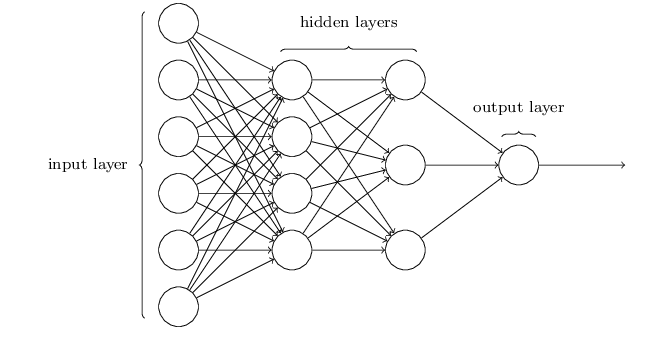
\includegraphics[width=1\linewidth]{project_2/figures/generic_NN.png}
    \caption{Illustration of a generic neural network. \cite[Taken from][The architecture of neural networks]{nielsen}.}
    \label{fig:NN}
\end{figure}

A general NN consists of an input layer, $k$ hidden layers and an output layer - all consisting of a varying number of nodes, as visualized in Fig. \ref{fig:NN}. The number of nodes in a layer is denoted as the width of the layer, and the number of layers in a network is denoted the depth of the network. 
Hidden layers are not hidden in the sense that they're not a visible part of the model; but rather that when using a trained model one never interacts with anything past the input and output layers, thus the internal nodes appear as hidden. 
Between the nodes we have connections called \textit{weights}. These determine the influence from one particular node to another. 

The weighted model stems from the mathematical function for an artificial neuron given as follows; 

\begin{equation}\label{artifical_neuron}
    y = f\left( \sum_{i=0}^Nwx_i \right) 
\end{equation}

Here $f$ is some \textit{activation function} that takes a weighted sum of $N$ inputs and maps them to an output. 
It is sometimes specified wether a network is \textit{fully connected} or not. A fully connected network, or layer, is simply connected in a way that each node receives the output from every single node in the preceding layer. Fig. \ref{fig:NN} is an example of a fully connected NN. However, a fully connected network can always act as a "not-fully connected" network simply by having some of it's weight set to $0$ and thereby nullifying the corresponding connections. 

The simplest model for an artificial neural network is called a \textit{feed forward neural network} (FFNN), where logically enough the flow of information moves only in one direction; forward. Consider for instance a FFNN with one hidden layers. The input-layer receives the input $X$, which is then passed through the first weights $W_0$ to the second layer. Here the weighted sum is passed through an activation function $f$ and passed via $W_1$ to the output layer. In the output layer the weighted sum is passed through $f$ one last time, before finally being output from the model. For each node $n$ in the first layer this process can be formally expressed as:


\begin{equation}
    y = f\left( \sum_{i=0}^N w_{0n}x_i + b\right)
\end{equation}
\citep[p.17]{Ketkar2017}. Here one can clearly see the similarities to Eq. \ref{artifical_neuron}. $b$ represents what is called a \textit{bias term}. Looking back to the structural similarities of a biological NN, the bias allows one to skew "how easy it is to get the neurons to fire". I.e., by altering the bias terms one can shift the the output values in a desired direction - in theory. This is however easier said than done, and directly altering either weights or biases directly are not common procedure. Instead one relies on a good choice of cost function and the training of the NN to produce fitting parameters. 

\subsubsection{Training of the network}
To start training the NN, and navigating the landscape of the cost-function one needs a starting point. For initialization of weights and biases there are a lot of different conventions. Arguably the most common across the field, is random initialization. As the wording entails, they're then randomly initialized. 
- Weights and biases
    - How they are initialized
Finnes spesialiserte metoder 

Choice of cost function

Back propagation process (refer to GD/cost functions)

\subsubsection{Activation functions}
Why they should not be linear

Examples: sigmoid, ReLU, leaky ReLU, softmax, identity in last layer?
% - Why neural networks
% - 
% \julie{need motivation for NN, one direction FF no loops, input-hidden-output}
% - Backprop
% - The choice of cost function
% - Hidden layers and nodes
% - Activation functions: sigmoid, ReLU, leaky ReLU
% - Should specify why it is important that the activation functions are non-linear
% - Activation function for final layer depends on the application, i.e. regression versus classification
% - Weights and their initialization
% - Initialization of biases  

% \subsection{Resampling methods\mia{copy}}


% When training models, error estimation is crucial both for model selection and model assessment. Without a good metric for the performance of the model it is impossible to gauge how well fit a model actually is.
% Generally, it's desirable to have as much data as possible for the training of a model. When holding off some of the data for testing, this data can then not be used for training. It's therefore of interest to explore methods that allow for a train-test split of the data, while still keeping as much data as possible for training and giving us a better error estimation.

% \subsubsection{Bootstrapping\mia{copy}}
% Bootstrapping is a general term for one such resampling method where one draws with replacement from the original data set, creating a "new" data set for each bootstrap. Every bootstrap sample should have the same size as the original data set, $n$. $B$ such samples are generated, and the training repeated for each of them.
% The $b$-th bootstrap sample produces model $\hat{f}_b$ \citep[p. 249]{hastie}.

% Using bootstrap the estimation of the error can be calculated as follows:
% %the mean of the error across the $B$ bootstrap samples \cite[p. 250]{hastie}:

% \begin{equation}\label{bs_error}
%     BS_{error} = \frac{1}{n}\sum_{i=0}^{n-1} L\left(y_i,\frac{1}{B}\sum_{b=1}^{B} \hat{f}_b(x_i)\right)
% \end{equation}

% \subsubsection{K-fold cross-validation\mia{copy}}
% \textit{K-fold cross-validation} is another method of resampling. 
% The data set is divided into $K$ parts $\mathcal{F}_k$, called folds. 
% The $K$ must be chosen by the developer as they see fit. 
% $K-1$ folds are used as training data, while the remaining fold is used as test data. The model trained when the $k$-th fold is held out, is denoted $f^{k}$. 
% The procedure is repeated $K$ times, holding out a new fold each time. For k-fold cross-validation the estimated error is given as the mean of the $K$ test errors, shown in Eq. \ref{cv_error} \citep[p. 241]{hastie}. Her one takes into consideration that the folds $\mathcal{F}_k$ may be of different sizes.


% \begin{equation}\label{cv_error}
%     CV_{error} = \frac{1}{K} \sum_{k=1}^{K} \frac{1}{|\mathcal{F}_k|} \sum_{i \in \mathcal{F}_k} L\left(y_i, f^{k}({x}_i)\right) 
% \end{equation}

% There are both advantages and disadvantages of this method. On one hand, it achieves the goal of maintaining a train-test split while keeping a sizeable train set. 
% The estimated error (Eq. \ref{cv_error}) will be closer to the true generalization error measure. This is a consequence of the error being averaged over many different models, and thereby to a higher degree taking into account randomness associated with data-selection. 

% On the other hand, cross-validation will be quite computationally costly for a high $K$. Another disadvantage is that there is no clear choice of $K$; here there is a trade-off between bias and variance. A smaller K leads to lower variance, but higher bias. On the other side, a higher K leads to low bias, but high variance. The extreme case of the latter is leave-out-one cross-validation (LOOCV), where every datapoint acts as a fold. It will lead to an unbiased error measure, but the variance will be quite large \citep[p. 242]{hastie}.


\subsection{Evaluation measures\mia{copy}}

\subsubsection{Regression}
The \emph{mean squared error} (MSE) is a popular error measure for linear regression models, and is defined as: 

\begin{equation}\label{mse}
    \text{MSE} = \frac{1}{n}\sum_{i=0}^{n-1}(y_i-\Tilde{y}_i)^2.
\end{equation}

$n$ denotes the number of data points in the training data, and the prediction for the i-th data point is denoted $\Tilde{y}_i$. Comparing the expression above to Eq. \ref{cost_ols}, it's clear how the OLS regression method is inherently designed to minimize MSE. 
% Given a loss-function of the squared distance between the prediction and the true value, the errors for cross-validation and bootstrapping (respectively Eq. \ref{cv_error} and Eq. \ref{bs_error}) will trivially be the equivalent of MSE. 

$R^2$ is a measure of how well the model explains the variance present in the data. 
\begin{equation}
    R^2 = 1 - \frac{RSS}{TSS}= 1 - \frac{\sum_{i=0}^{n-1}(y_i-\Tilde{y}_i)^2}{\sum_{i=0}^{n-1}(y_i-\overline{y}_i)^2},
\end{equation}

$R^2 \in (-\infty,1]$. If $R^2 = 1$ the model perfectly explains all variance, whereas a value of 0 would mean does not explain any of the variance. 
A prediction $\tilde \y = \bar \y$, would result in $R^2 = 0$.
If $R^2<0$, the model is worse than a straight line.
The numerator is the sum of the squared residuals, also called RSS. The denominator is the total sum of squares, in short TSS \cite[p. 29]{martin}.

\subsubsection{Classification}
While the mean squared errors and $R^2$ measures still tells us something about the quality of a classification model, there are several other methods which can better measure the model's performance.
One such measure is \textit{accuracy}.
\begin{equation}\label{eq:acc}
    \text{accuracy} = \frac{\text{correct predictions}}{\text{total predictions}}
\end{equation}
Accuracy is simply defined as correct predictions divided by total predictions (see Eq. \ref{eq:acc}), and is a good measure on how often the model is correct.
There is an important weakness with accuracy, especially when considering certain types of data.
This stems from the fact that the two types of errors in a binary classification model, \textit{false positives} and \textit{false negatives}, are in many cases not equally bad.
A prime example of this is models based on medical data sets, trying to predict whether a patient has some disease, such as the Wisconsin breast cancer data set \cite{breast_cancer_wisconsin}.
Clearly, in most these cases, it is worse if the models wrongly predict that a sick patient is healthy, than the other way around.
\begin{table}[h]
    \centering
    \begin{tabular}{|m{8em}|m{8em}|m{8em}|}
    \hline
         & \textbf{predicted to have the disease} & \textbf{predicted to not have the disease} \\
         \hline
         \textbf{has disease} & true positive & false negative \\
         \hline
         \textbf{not disease} & false positive & true negative\\
    \hline
    \end{tabular}
    \caption{Confusion matrix for medical data}
    \label{tab:my_label}
\end{table}

An example is the 

\subsection{\mia{MIA THINGS}}

sigmoid, softmax, relu, leakyrelu
mse, binary cross-entropy 

\gaute{ clipping grads }

minmax scaler + benefits of the different scalers 

logreg 

accuracy

manual grads

chain rule 

\gaute{constant, momentum, adagrad, adagrad momentum, adam, rmsprop }

recall, precision, ROC, confusion matrix 
    why standard accuracy is bad for medical data
